\section{Classification}

\begin{frame}[standout]{\currentname: Problem Description}
    Goal: predict the presence of a fatality in a gun incident.
\end{frame}

\begin{frame}<1-5>{\currentname: Feature Selection}
    \begin{exampleblock}{\textsc{Obvious Features to Remove}}
        All features directly related to the target variable.
    \end{exampleblock}
    \begin{exampleblock}<2->{\textsc{Less Obvious}}
        \begin{itemize}
            \item n\_killed = {\only<3->{\color{red}}n\_participants} - n\_injured - n\_unharmed - n\_arrested
            \item n\_participants = {\only<4->{\color{red}}n\_males} + n\_females
            \item n\_participants = {\only<4->{\color{red}}n\_adult} + n\_teen + n\_child
        \end{itemize}
    \end{exampleblock}
    \begin{exampleblock}<5->{\textsc{Lesser Obvious Problem}}
        $\sim50\%$ of datapoints have n\_participants = 1.
    \end{exampleblock}
\end{frame}

\begin{frame}{\currentname: Data Preparation}
    \begin{exampleblock}{\textsc{Scaling}}
        \vspace*{0.5em}
        StandardScaler from sklearn.
    \end{exampleblock}
    \begin{exampleblock}{\textsc{Train-Valid-Test Splits}}
        \vspace*{-1em}
        \begin{flalign*}
            \text{Train} &= 70\%& \\
            \text{Valid} &= 15\%& \\
            \text{Test}  &= 15\%&
        \end{flalign*}
    \end{exampleblock}
    \vspace*{-1em}
    \begin{exampleblock}{\textsc{Balancing}}
        \vspace*{0.5em}
        $75\%$ of 0-labelled datapoints. \\
        \vspace*{0.5em}
        \begin{minipage}{0.47\textwidth}
            Training balanced with SMOTE.
        \end{minipage}
        \begin{minipage}{0.47\textwidth}
            Validation and test balanced with random sampling with replacement.
        \end{minipage}
    \end{exampleblock}
\end{frame}

\begin{frame}{\currentname: Models}
    \begin{exampleblock}{Decision Tree}
        \begin{itemize}
            \item[] 16 levels
            \item[] Gini criterion
            \item[] 2 minimum samples per leaf
            \item[] 1 minimum sample per split
        \end{itemize}
    \end{exampleblock}
    \begin{exampleblock}{Neural Network}
        \begin{itemize}
            \item[] 4 hidden layers
            \item[] [32, 16, 8, 4] neurons per layer
            \item[] Sigmoid activation
            \item[] 0.1 dropout
        \end{itemize}
    \end{exampleblock}
\end{frame}

\begin{frame}{\currentname: Decision Tree Results I}
    \begin{figure}
        \centering
        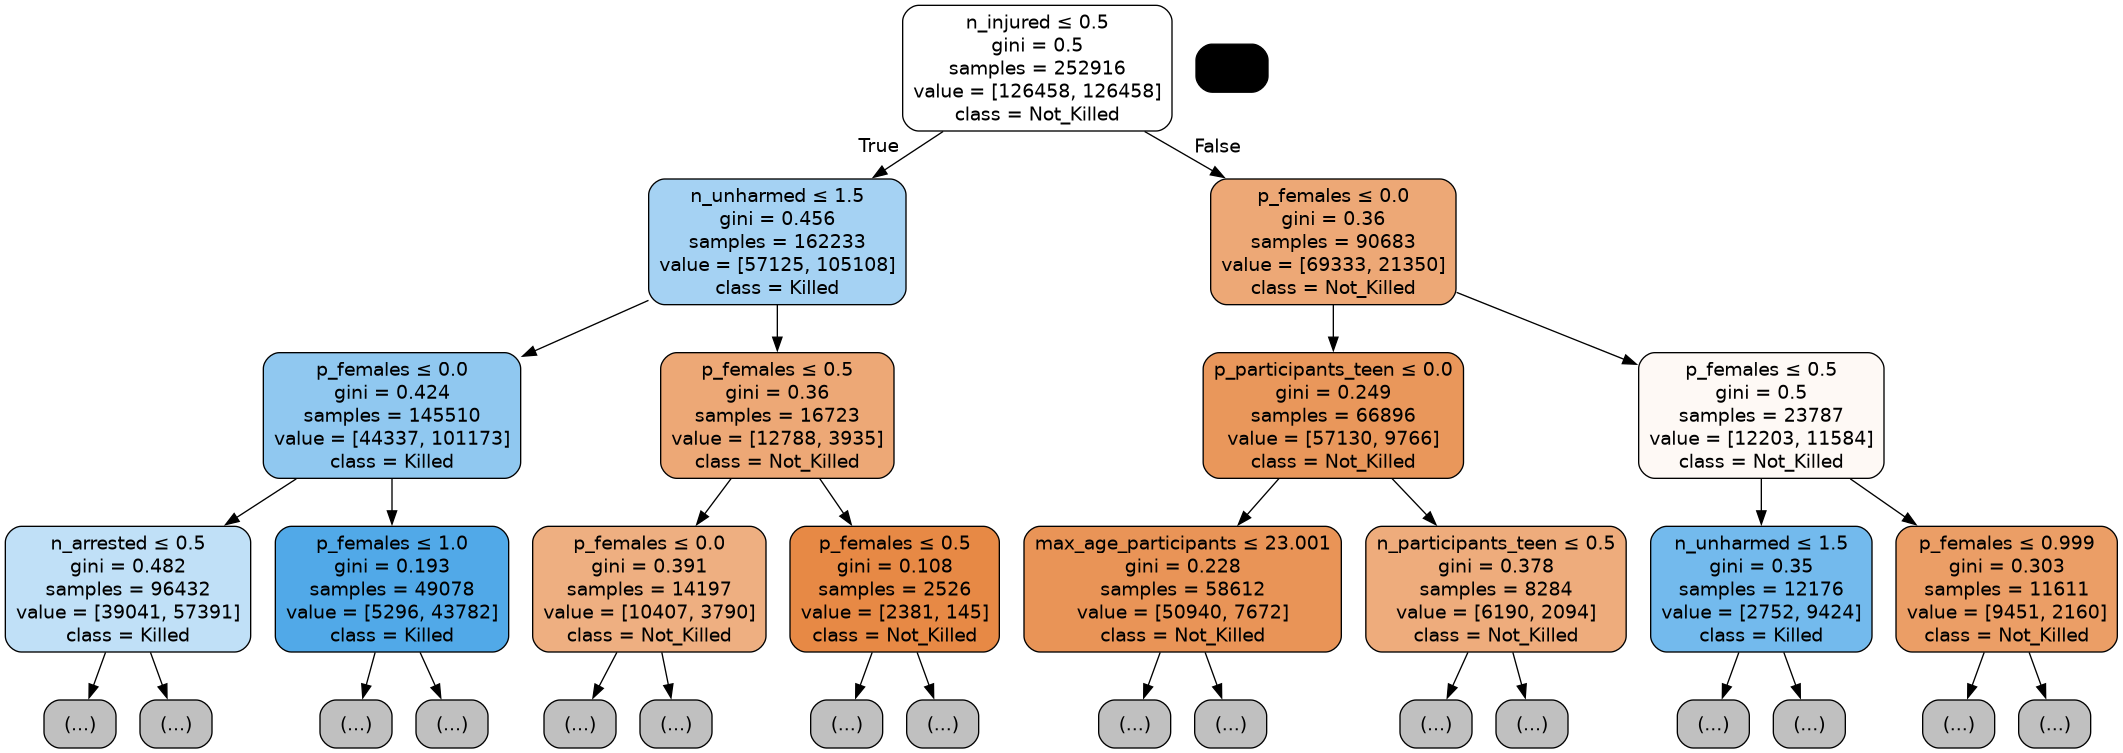
\includegraphics[width=.99\textwidth]{CS/decision_tree.png}
        \caption*{First 4 levels of the decision tree.}
    \end{figure}
\end{frame}

\begin{frame}{\currentname: Decision Tree Results II}
    \begin{figure}
        \centering
        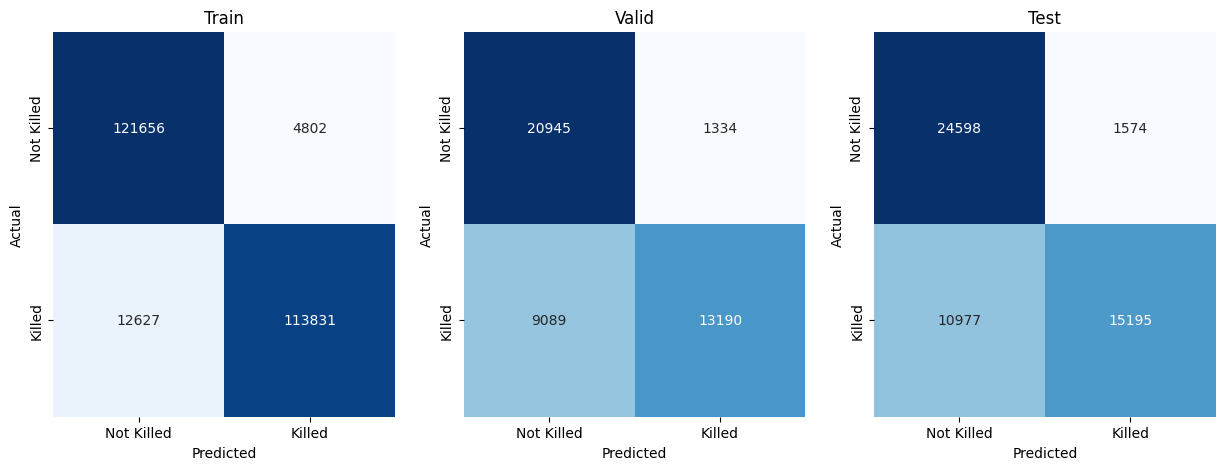
\includegraphics[width=.99\textwidth]{CS/decision_tree_cm.png}
        \caption*{Confusion matrix of the decision tree in TR/VL/TE splits.}
    \end{figure}
    \begin{table}[h]
        \centering
        \begin{tabular}{l|c|c|c|}
            Split & Train & Valid & Test \\
            \hline
            Accuracy  & 0.93 & 0.77 & 0.76 \\
            Precision & 0.96 & 0.94 & 0.94 \\
            Recall    & 0.90 & 0.70 & 0.70 \\
            F1        & 0.93 & 0.80 & 0.77 \\        
        \end{tabular}
    \end{table}
\end{frame}

\begin{frame}{\currentname: Neural Network Results}
    \begin{figure}
        \centering
        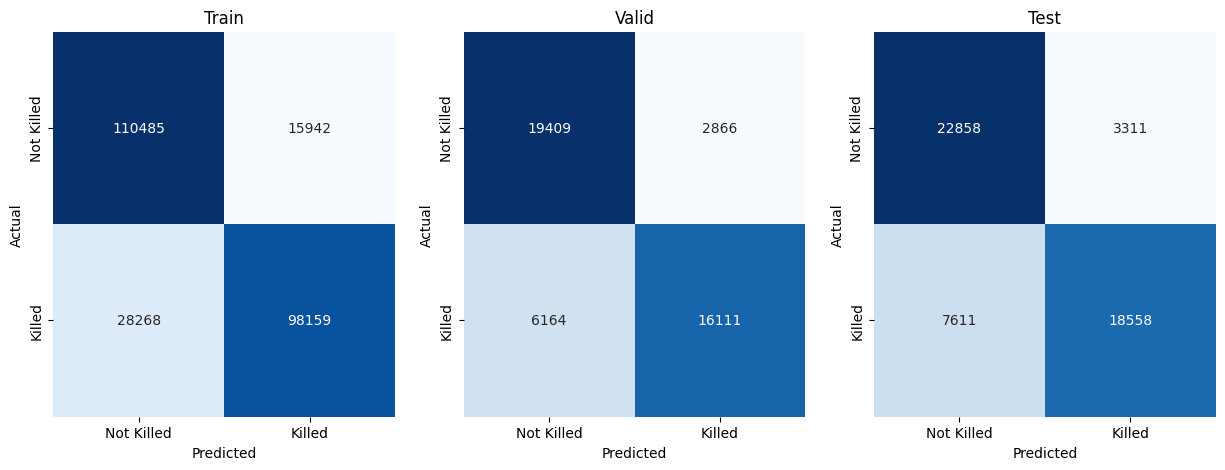
\includegraphics[width=.99\textwidth]{CS/nn_cm.png}
        \caption*{Confusion matrix of the Neural Network in TR/VL/TE splits.}
    \end{figure}    
    \begin{table}[h]
        \centering
        \begin{tabular}{l|c|c|c|}
            Split & Train & Valid & Test \\
            \hline
            Accuracy  & 0.83 & 0.80 & 0.79 \\
            Precision & 0.87 & 0.87 & 0.87 \\
            Recall    & 0.80 & 0.76 & 0.75 \\
            F1        & 0.83 & 0.81 & 0.81 \\        
        \end{tabular}
    \end{table}
\end{frame}

\begin{frame}{\currentname: Models Comparison}
    \begin{figure}
        \centering
        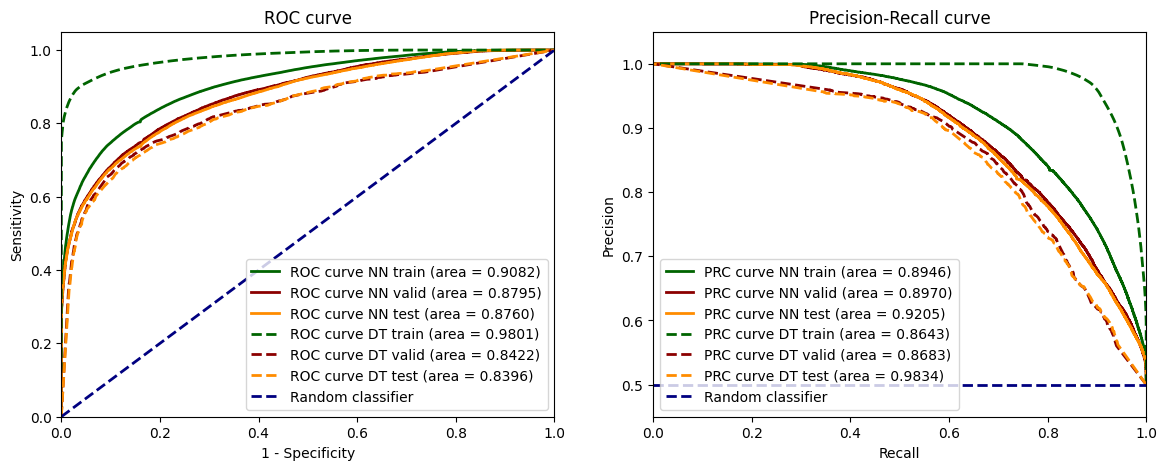
\includegraphics[width=.99\textwidth]{CS/roc-prc.png}
        \caption*{ROC/PRC curves of the two models in TR/VL/TE splits.}
    \end{figure}
\end{frame}